\chapter{非线性差分方程的精确解和N阶展开方法的推广}
\section{Introduction}\label{Introduction-02}

Searching exact solutions of difference equations is a major aspect in the studies of computer algebra. Difference equation is also called recurrence equation. The simplest form of difference equation is a linear equation with constant coefficients, i.e.,
\begin{equation}
\sum_{k=0}^l{c_k f(x+k)}=g(x).
\label{ceq}
\end{equation}
Here $f(x)$ is the undetermined function, $g(x)$ is an arbitrary function, and $c_k (k=1,\cdots,l)$ are constants. The solution of \refeqn{ceq} had been solved long times ago.  A simple extension of \refeqn{ceq}  is linear equation with polynomial coefficients, i.e.,
\begin{equation}
\sum_{k=0}^l{p_k(x)f(x+k)=p_{l+1}(x)},
\label{peq}
\end{equation}
in which $p_k(x) (k=1,\cdots,l+1)$ are polynomials. The research for \refeqn{peq} was started about 30 years ago. In 1989, Abramov first considered \refeqn{peq} and proposed an algorithm to find all polynomial solutions\citep{Abramov1989polynomial}. In the same year, Abramov developed an algorithm to find the universal denominator of all rational solutions, then the rational solution of \refeqn{peq} was solved\citep{Abramov1989rational}. In 1992, \Petkovsek{} proposed an algorithm to find the hypergeometric solution\citep{petkovvsek1992hypergeometric}. The division of two items in hypergeometric solution is a rational function. Applying shift and partial sum on hypergeometric solution can generate d'Alembertian solutions. The d'Alembertian solution of \refeqn{peq} was solved by Abramov and \Petkovsek{} in 1994\citep{abramov1994dAlembertian}. Applying shift, partial sum and interlacing on d'Alembertian solution can generate Liouvillian solutions. The Liouvillian solution of \refeqn{peq} was solved in 1999 by Hendricks and Singer\citep{hendricks1999Liouvillian}.

Since then, the type of solutions has not been extended, but the algorithm has been updated for several generations. Some improvement extended the applicable equations from difference equations to q-difference equations and differential equations. For example, \cite{Abramov1995polynomial} is an extension for polynomial solutions, \cite{Abramov1995Rational} is an extension for rational solutions. Other updates have improved the efficiency of the algorithms. For example, \cite{ud2007,ud2010,ud2011,ud2012} is a series of work to optimize the algorithm of finding universal denominators for rational solutions, which is the most expansive part in the solving procedure.

Starting with the polynomial solution, the solvable solution of \refeqn{peq} is becoming more and more general. However, all solutions of \refeqn{peq} have not been completely solved. Inspired by the development of solving linear difference equation with polynomial coefficients, we decide to find polynomial solutions of nonlinear difference equation with polynomial coefficients. As an extension of \refeqn{peq}, we consider the nonlinear difference equation in the form of
\begin{equation}
\sum_{k=0}^l{\mbrace{a_k(x)\prod_{i=0}^r{f^{\gamma_{ki}}(x+i)}}}=0.
\label{eq}
\end{equation}
Here, $K$ is a field,  $a_k(x)\in K[x], l>1, \gamma_{ki}\ge 0$. The purpose of this paper is to find all polynomial solutions of \refeqn{eq}.

The solving of differential equations has much more abundant research results than that of difference equations. Homogeneous balance principle has been widely applied in the solving of differential equations. This principle arises from the idea that the highest order items in an equation are balanced under certain aspect. Since this principle was proposed\citep{wang1995solitary,wang1996application}, it has been applied to construct solutions of various kinds of differential equations\citep{hbAppl2006,hbAppl2009a,hbAppl2009b,hbAppl2010}. It is a direct and algebraic approach, many methods based on it have implemented programs, such as \cite{li2002rath} and \cite{li2004raeem}.

Inspired by the application of homogeneous balance principle in differential equations, we decide to apply it in seeking polynomial solutions of \refeqn{eq}. However, the homogeneous balance principle works only in some cases. Hence, we propose a new $n$-order expansion method to process the rest cases.

The paper is organized as follows. In \refsec{Homogeneous-02} we use the homogeneous balance principle to solve \refeqn{eq} in some cases. In \refsec{Expansion-02} a new $n$-order expansion method is proposed to solve the rest cases of \refeqn{eq}. In \refsec{visualization-02}, a visual summary of the two methods is presented. We also provide several typical examples to show how our method works. The implementation of the algorithm is described in \refsec{implementation-02}. Experiments in \refsec{Experiments-02} show the effectiveness and efficiency of our algorithm. In \refsec{$n$-order-discussion-02},  a further discussion about the effectiveness of our algorithm is provided theoretically. Finally, conclusions are given in \refsec{Conclusion-02}.


\section{Homogeneous balance principle}\label{Homogeneous-02}

Assuming
\begin{equation}
f(x)=\sum_{k=0}^m{\mu_kx^k},
\label{fm1}
\end{equation}
we can find all polynomial solutions of \refeqn{eq}, whose degree is no more than $m$, by the method of undetermined coefficients. In order to find all polynomial solutions, we need to determine the upper bound of $m$.

Substitute \refeqn{fm1} into \refeqn{eq}, the left side of the equation is still a polynomial, we can extract degrees of different items to form a list
\begin{equation}
D = \mbrace{s_1 m+d_1,s_2 m+d_2,\cdots,s_l m+d_l},
\end{equation}
where
\begin{equation}
\begin{split}
s_k&=\sum_{i=0}^r{\gamma_{ki}}, \\
d_k&=\deg a_k(x).
\end{split}
\label{eq-sd}
\end{equation}
Each degree in $D$ is the a linear expression of $m$, which is called the \emph{order} of the corresponding item.

The obtained polynomial is equal to zero requires that the combined coefficient of all the highest order items equals to zero. Because each highest item is nonzero, there must be more than two different items have the same degree and their coefficients can be added to zero. Thus, the following constraints must be satisfied
\begin{equation}
\left\{
\begin{array}{l}
m\in \mathbb Z_+  ,                                     \\
\exists i\neq j, s_i m+d_i=s_j m+d_j    ,               \\
\forall k \not\in \bbrace{i,j}, s_i m+d_i\ge s_k m+d_k .
\end{array}
\right.
\label{cond}
\end{equation}
These three constraints are called \emph{integer constraint}, \emph{balance constraint} and \emph{maximum constraint}, respectively.

(I) When $s_i \neq s_j$, we can get
\begin{equation}
m=\frac{d_j-d_i}{s_i-s_j}.
\end{equation}
If $m$ satisfy the rest constraints in \refeqn{cond}, it can be called as \BPone{} (balance points of the first kind). We represent the set of them as
\begin{equation}
M_1=\bbrace{\left. m=\frac{d_j-d_i}{s_i-s_j}\in \mathbb Z_+\right\vert \forall k\not\in \bbrace{i,j}, s_i m+d_i\ge s_k m+d_k}.
\end{equation}

(II) When $s_i = s_j$, the \emph{balance constraint} is always satisfied. Consider the \emph{maximum constraint}, we can get
\begin{equation}
\left\{
\begin{split}
m > \frac{d_k-d_i}{s_i-s_k}, & \text{ if } s_i>s_k,  \\
m < \frac{d_k-d_i}{s_i-s_k}, & \text{ if } s_i<s_k.  \\
\end{split}
\right.
\end{equation}
The equality condition has been eliminated due to the condition of \BPone{}. Thus, we have
\begin{equation}
\underset{s_i>s_k}{\max}{\frac{d_k-d_i}{s_i-s_k}} < m < \underset{s_i<s_k}{\min}{\frac{d_k-d_i}{s_i-s_k}}.
\end{equation}
The undetermined degree $m$ would have upper bound when $s_i m + d_i < \sigma m + \delta$. Here
\begin{equation}
\begin{split}
\sigma &= \max ~s_k,  \\
\delta &= \underset{s_k=\sigma}{\max}{~d_k}.
\end{split}
\label{eq-max-sd}
\end{equation}

In the light of the bounds of $m$, there are two cases to be considered.

(II-a) When $s_i m + d_i < \sigma m + \delta$, $m$ has limited possible values. We call them as \BPtwo{} (balance point of the second kind), and represent them as
\begin{equation}
M_2=\bbrace{m\in \mathbb Z_+\left|\underset{s_i>s_k}{\max}{\frac{d_k-d_i}{s_i-s_k}} < m < \underset{s_i<s_k}{\min}{\frac{d_k-d_i}{s_i-s_k}}\right.} .
\end{equation}

(II-b) When $s_i m + d_i = \sigma m + \delta$, we cannot determine the upper bound of $m$ by the homogeneous balance principle. So, we propose a novel \emph{$n$-order expansion method}.

\section{N-order expansion method}\label{Expansion-02}

The homogeneous balance principle only consider orders of the highest items, we propose a novel \emph{$n$-order expansion method} by take the coefficients of the highest $n$ items into account.

Given $n>0$, define an \emph{$n$-order expanded polynomial} of degree $m$ is
\begin{equation}
F\sbrace{x,m,u\up n}=\sum_{k=0}^{n-1}{u_k x^{m-k}}+\OO\sbrace{x^{m-n}},
\label{npoly}
\end{equation}
where $u\up n=\mbrace{u_0,u_1,\cdots,u_{n-1}}$ is the vector of coefficients, and
\begin{equation}
\OO\sbrace{x^n}=\left\{
\begin{array}{cl}
\text{polynomials of degree that no more than } n & n\ge 0, \\
0                                                 & n<0 .
\end{array}
\right.
\end{equation}

For the undetermined polynomial $f(x)$ of degree $m$, assuming the coefficient vector of the highest $n$ items is $u\up n=\mbrace{u_0,u_1,\cdots,u_{n-1}}$, we have
\begin{equation}
f(x)=F\sbrace{x,m,u\up n}.
\end{equation}

For the coefficient polynomial
\begin{equation}
a_k(x)=\sum_{i=0}^{d_k}{a_{k,i} x^{d_k-i}},
\end{equation}
we assume that
\begin{equation}
\alpha_{k,i}=\left\{
\begin{array}{cl}
a_{k,i} & i\le \min\{n-1,d_k\}, \\
0       & i >  \min\{n-1,d_k\},
\end{array}
\right.
\end{equation}
and have
\begin{equation}
a_k(x)=F\sbrace{x,d_k,\alpha_k\up n},
\end{equation}
where $\alpha_k\up n=\mbrace{\alpha_{k,0},\alpha_{k,1},\cdots,\alpha_{k,n-1}}$.

Thus, we can rewrite the \refeqn{eq} in the form of \emph{$n$-order expanded polynomial} after the fundamental operations have been inferred.

Firstly, we consider the shift operation
\begin{equation}
\Delta^r F\sbrace{x,m,u\up n} = F\sbrace{x+r,m,u\up n} = f(x+r).
\end{equation}
When $r\neq 0$, we have
\begin{equation}
\begin{split}
\Delta^r F\sbrace{x,m,u\up n} &= \sum_{k=0}^{n-1}{u_k (x+r)^{m-k}}+\OO\sbrace{x^{m-n}} \\
&= \sum_{k=0}^{n-1}{u_k \mbrace{\sum_{j=0}^{m-k}{\binom{m-k}{j}r^kx^{m-k-j}}}}+\OO\sbrace{x^{m-n}} \\
&= \sum_{k=0}^{n-1}{u_k \mbrace{\sum_{m-k-j>m-n}{\binom{m-k}{j}r^kx^{m-k-j}}}}+\OO\sbrace{x^{m-n}} \\
&= \sum_{k+j<n}{u_k {\binom{m-k}{j}r^kx^{m-k-j}}}+\OO\sbrace{x^{m-n}} \\
&=\sum_{p=0}^{n-1}{x^{m-p}\mbrace{\sum_{k=0}^p{u_k\binom{m-k}{p-k}r^{p-k}}}}+\OO\sbrace{x^{m-n}}\\
&=F\sbrace{x,m,v\up n}.
\end{split}
\end{equation}
Here $v\up n=\mbrace{v_0,v_1,\cdots,v_{n-1}}$, and
\begin{equation}
v_p=\sum_{k=0}^p{u_k\binom{m-k}{p-k}r^{p-k}}.
\end{equation}

Notice that the coefficient $v_p$ is a polynomial with respect to $m$, we can not only determine $m$ by orders, but also determine it by coefficients.

Secondly, consider the multiply operation
\begin{equation}
\begin{split}
& F\sbrace{x,m,u \up n}\cdot F\sbrace{x,l,v\up n} \\
=& \mbrace{\sum_{k=0}^{n-1}{u_k x^{m-k}}+\OO\sbrace{x^{m-n}}}\mbrace{\sum_{k=0}^{n-1}{v_k x^{l-k}}+\OO\sbrace{x^{l-n}}} \\
=& \mbrace{\sum_{k=0}^{n-1}{u_k x^{m-k}}}\mbrace{\sum_{k=0}^{n-1}{v_k x^{l-k}}}+\OO\sbrace{x^{m+l-n}} \\
=& \sum_{p=0}^{n-1}{x^{m+l-p}\mbrace{\sum_{k=0}^p{u_k v_{p-k}}}}+\OO\sbrace{x^{m+l-n}} \\
=& F\sbrace{x,m+l,w\up n} .
\end{split}
\end{equation}
Here $w\up n=\mbrace{w_0,w_1,\cdots,w_{n-1}}$, and
\begin{equation}
w_p=\sum_{k=0}^p{u_k v_{p-k}}.
\end{equation}

Thus, we can rewrite each item in the form of \emph{$n$-order expanded polynomial}, i.e.,
\begin{equation}
\begin{split}
a_k(x)\prod_{i=0}^r{f^{\alpha_{ki}}(x+r)}&=F\sbrace{x,d_k,\alpha_k\up n}\prod_{i=0}^r{\Delta^{\gamma_{ki}}F\sbrace{x,m,u\up n}} \\
&= F\sbrace{x,s_k m+d_k, \omega_k\up n} .
\end{split}
\end{equation}

Finally, consider the add operation
\begin{equation}
F\sbrace{x,s_i m+d_i,u\up n}+F\sbrace{x,s_j m+d_j,v\up n},
\end{equation}
which is much more complicated. In general, we cannot compare $s_i m + d_i$ with $s_j m + d_j$ when $m$ is undetermined. Assuming
\begin{equation}
s_i m+d_i\ge s_j m+d_j+n, \label{cond_add}
\end{equation}
we have
\begin{equation}
\begin{split}
&F\sbrace{x,s_i m+d_i,u\up n}+F\sbrace{x,s_j m+d_j,v\up n} \\
=&\left\{
\begin{array}{cl}
    F\sbrace{x,s_i m+d_i,u\up n} & s_i>s_j ,            \\
    F\sbrace{x,s_i m+d_i,w\up n} & s_i=s_j,d_i\ge d_j .
\end{array}
\right.
\end{split}
\end{equation}
Here,
\begin{equation}
w_p=\left\{
\begin{array}{cl}
u_p               & p<d_i-d_j ,   \\
u_p+v_{p-d_i+d_j} & p\ge d_i-d_j.
\end{array}
\right.
\end{equation}

Finally, \refeqn{eq} can be rewritten as
\begin{equation}
F(x,\sigma m + \delta,\Omega\up n)=0,
\label{eq-np}
\end{equation}
where $\Omega\up n=\mbrace{\Omega_0,\cdots,\Omega_{n-1}}$, and $\Omega_k$ is a polynomial with respect to $m$ and $u_k$.

Under the situation (II-b), according to \refeqn{cond_add}, the $k$-th ($k=0,1,\cdots$) coefficient in \refeqn{eq-np} requires that
\begin{equation}
\forall s_j<\sigma, \sigma m + \delta - k > s_j m + d_j,
\end{equation}
i.e.,
\begin{equation}
m > \underline{m}_k=\underset{s_j<\sigma}{\max}{\frac{d_j-\delta+k}{\sigma-s_j}}.
\end{equation}

Now we can find a new kind of balance point called \BPthree{} (balance points of the third kind). Because the left side of \refeqn{eq} is not a constant, there must be $\Omega_k\neq 0$ when $n$ is big enough. Assume that $\Omega_{k_0}$ is the first nonzero item. 

If $\bbrace{\Omega_{k_0}=0,u_0\neq 0}$ has positive integer solution $m=m_0$, the degree of all polynomial solutions of \refeqn{eq} must be no more than $m_0$. Meanwhile, the validation of the $k_0$-th expansion requires $m>\underline{m}_{k_0}$. Then,  all \BPthree{} are in the set
\begin{equation}
M_3=\bbrace{m\in \mathbb Z_+|\max\sbrace{M_1\cup M_2 \cup \bbrace{\underline{m}_{k_0}}}<m\le m_0}.
\end{equation}

Otherwise, if $\bbrace{\Omega_{k_0}=0,u_0\neq 0}$ has no positive integer solution, it means that \refeqn{eq} has no polynomial solution when $m>\underline{m}_{k_0}$. In other words, the original equation may has polynomial solutions when $m\le \underline{m}_{k_0}$. So, all \BPthree{} are in the set
\begin{equation}
M_3=\bbrace{m\in \mathbb Z_+|\max\sbrace{M_1\cup M_2}<m\le \underline{m}_{k_0}}.
\end{equation}

Finally, we can determine the upper bound of degree $m$, i.e.,
\begin{equation}
\overline m =\max\sbrace{M_1\cup M_2\cup M_3}.
\end{equation}
Substitute $f(x)=\sum_{k=0}^{\overline m}{\mu_k x^k}$ into \refeqn{eq}, we can get all polynomial solutions.

\section{Method visualization and examples} \label{visualization-02}

In the previous sections, we have determined the upper bound of solution degree under three constraints in \refeqn{cond}. The order of each item in \refeqn{eq} is the a linear expression of $m$, and can be regarded as a line in the plane. The orders can be represented as
\begin{equation}
\lambda_1(m),\cdots,\lambda_l(m).
\end{equation}
Here $\lambda_k(m)=s_k m+d_k$. Our algorithm is equivalent to find integer intersection points of two or more different lines on the broken line
\begin{equation}
\lambda(m)=\max\bbrace{\lambda_1(m),\cdots,\lambda_l(m)}.
\end{equation}

For example, as shown in \reffig{point}, there are 7 lines that are marked as $\lambda_1,\cdots,\lambda_7$. Here, red means multiple and black means unique. The solid broken line represents $\lambda(m)$. There are 8 possible balance points that are marked as $B_1,\cdots,B_8$, respectively. Assuming that they are integer points.
\begin{figure}[H]
\centering
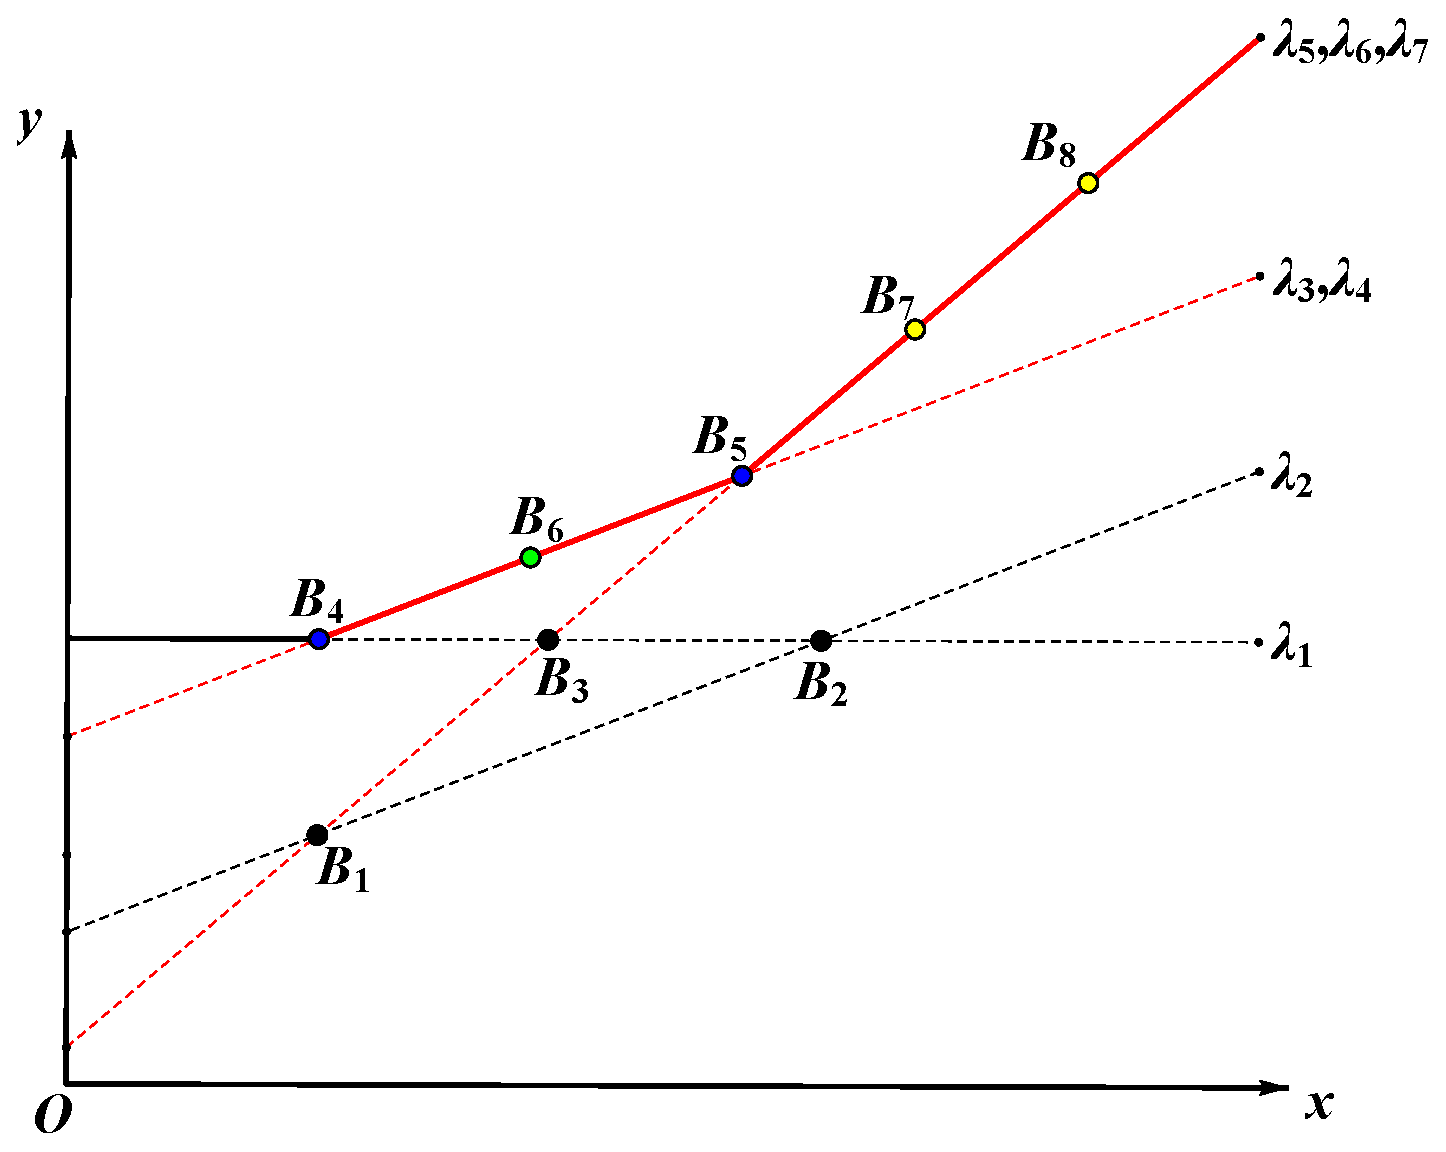
\includegraphics[width=0.6\textwidth]{fig/ps.eps}
\caption{Visualization of balance points}
\label{point}
\end{figure}
\begin{compactitem}[\textbullet]
\item However, $B_1,B_2$ and $B_3$ are the intersections of different lines, they don't meeting the maximum constraint, so they are not balance points.
\item $B_4$ and $B_5$ are the intersections of different lines and meeting the maximum constraint, so they are \BPone{}.
\item $B_6$ is not the intersection of different lines, but there are multiple lines go through it, and it is bounded by $B_4$ and $B_5$. So, it is \BPtwo{}.
\item $B_7,B_8$ and more integer points following them are possible \BPthree{}. They are not bounded by other balance points, but we can determine the veritable ones by the $n$-order expansion method.
\end{compactitem}



Here are some typical examples.

\begin{example}
(\BPone{})
\begin{equation}
-x^4f(x+3)+(x+1)f(x)^2+8x^6+27x^5+28x^4+2x^3-x-1=0 \label{ep1} .
\end{equation}

We can obtain the list of orders, i.e., $[m+4,2m+1,6]$. Since there is no identical order, this equation only has \BPone{}. From $m+4=6,2m+1=6$ and $m+4=2m+1$, we can get $M_1=\{2,3\}$ and $\overline m = 3$. Then, substitute $f(x)=\sum\nolimits_{k=0}^3{\mu_k x^k}$ into \refeqn{ep1}, we can get the polynomial equations of coefficients, i.e.,
\begin{equation}
\left\{
\begin{array}{l}
    {\mu_{{0}}}^{2}-1=0,                                                                                                  \\
    {\mu_{{3}}}^{2}-\mu_{{3}}=0,                                                                                            \\
    {\mu_{{0}}}^{2}+2\,\mu_{{0}}\mu_{{1}}-1=0,                                                                                \\
    2\,\mu_{{0}}\mu_{{1}}+2\,\mu_{{0}}\mu_{{2}}+{\mu_{{1}}}^{2}=0,                                                                \\
    2\,\mu_{{2}}\mu_{{3}}+{\mu_{{3}}}^{2}-\mu_{{2}}-9\,\mu_{{3}}+8=0,                                                             \\
    2\,\mu_{{0}}\mu_{{2}}+2\,\mu_{{0}}\mu_{{3}}+{\mu_{{1}}}^{2}+2\,\mu_{{1}}\mu_{{2}}+2=0,                                            \\
    2\,\mu_{{1}}\mu_{{3}}+{\mu_{{2}}}^{2}+2\,\mu_{{2}}\mu_{{3}}-\mu_{{1}}-6\,\mu_{{2}}-27\,\mu_{{3}}+27=0,                              \\
    2\,\mu_{{0}}\mu_{{3}}+2\,\mu_{{1}}\mu_{{2}}+2\,\mu_{{1}}\mu_{{3}}+{\mu_{{2}}}^{2}-\mu_{{0}}-3\,\mu_{{1}}-9\,\mu_{{2}}-27\,\mu_{{3}}+28=0.
\end{array}
\right.
\label{ceqs}
\end{equation}
The solution of \refeqn{ceqs} is $\{\mu_0=-1,\mu_1=0,\mu_2=0,\mu_3=1\}$. Finally, the polynomial solution of \refeqn{ep1} is $f(x)=x^3-1$.
\end{example}

\begin{example}
(\BPtwo{})
\begin{equation}
x^2f(x)f(x+1)f(x+2)+(1-x^9)f(x)+(x^4-x^9)f(x+1)+2x^9f(x+2)-\sum_{k=0}^{10}{c_k x^k}=0, \label{ep2}
\end{equation}
where $[c_0,\cdots,c_{10}]=[1,1,22,57,85,72,35,9,1,10,6]$. The list of orders is $[3m+2,m+9,m+9,m+9,10]$. We can get \BPone{} from $m+9=10$, i.e., $M_1=\{1\}$. Since the repeated order $m+9$ is not the order with maximum coefficient of $m$, this equation only has \BPtwo{}. From $\{m+9> 10,m+9> 3m+2\}$, we can get $m< 7/2$. Thus, $\overline m=3$, and we can get the final solution of \refeqn{ep2} by undetermined coefficient method, i.e., $f(x)=x^2+x+1$. Obviously, we cannot get the polynomial solution of this equation without \BPtwo{}.
\end{example}

\begin{example}
(\BPthree{}, 2-order expansion)
\begin{equation}
(x+2)f(x)-(x-1)f(x+1)=0. \label{ep3}
\end{equation}
Since the list of orders is $[m+1,m+1]$, this equation only has \BPthree{}. Using the 2-order expansion, i.e., substitute $f(x)=u_0 x^m + u_1 x^{m-1} + \OO(x^{m-2})$ into \refeqn{ep3}, we can get
\begin{equation}
(-u_0 m+3u_0)x^m+\OO(x^{m-1})=0.
\end{equation}
Since $u_0\neq 0$, from $-u_0 m+3u_0=0$, we can get $m=3$. Then, we have $f(x)=c(x^3-x)$ by the undetermined coefficient method, where $c$ is an arbitrary constant.
\end{example}

\begin{example}
(\BPthree{}, high-order expansion)
\begin{equation}
-2x^5f(x)f(x+2)+x^4f(x)^2+(2x^5-x^4)f(x+1)^2-\sum_{k=0}^{22}{c_k x^k}=0, \label{ep4}
\end{equation}
where $[c_0,\cdots,c_{22}]=$[0, 0, 0, 0, 1, 2046, 10140, 22340, 28095, 20730, 7788, 6120, 30600, 84180, 151164, 199504, 199710, 151380, 85560, 35136, 10035, 1830, 170]. Here, the list of orders is $[2m+5,2m+4,2m+5,22]$. Since $2m+5=22\Rightarrow m=17/2$, this equation only has \BPthree{}. The first nonzero item in the $n$-order expansion is
\begin{equation}
\Omega_3 = 2m^2u_0^2-3mu_0^2-2u_0u_1.
\end{equation}
There is no positive integer solution of $m$. It means that there is no polynomial solution when $2m+5 > 22+3$. In other words, polynomial solution requires $m\le 10$. Thus, $\overline m =10$. Then the solutions of \refeqn{ep4} are $f(x)=\pm (x^{10}-1)$.
\end{example}

\begin{example}
(Application, 2-order expansion)

Consider the summation 
\begin{equation}
    S(x)=\sum_{k=0}^x{k^{10}}.
\end{equation}
We can construct a difference equation  
\begin{equation}
    S(x)-S(x-1)=x^{10}, S(0)=0. \label{seq}
\end{equation}
The list of orders is $\mbrace{m,m,10}$. Here, $m=10$ is \BPone{}. Since there are two $m$ in the list, \BPthree{} need to be considered. The 2-order expansion of this equation is 
\begin{equation}
u_0m x^{m-1}+\OO(x^{m-2})=0.   
\end{equation}
Because $u_0\neq 0$, $m$ must be 0 when $m-1>10$. So, $m\le 11$. Thus, $\overline m=11$. We can get the solution that
\begin{equation}
S(x)=\frac{5}{66}x-\frac{1}{2}x^3+x^5-x^7+\frac{5}{6}x^9+\frac{1}{2}x^{10}+\frac{1}{11}x^{11}.
\end{equation}
As we can see, the degree of solution is 11, while \BPone{} is 10. Hence, we cannot get this solution without 2-order expansion. 

Since the \refeqn{seq} is a linear equation, which can be solved by other methods, such as methods in \cite{Abramov1989polynomial} and \cite{Abramov1995polynomial}. But in our algorithm, it was solved by 2-order expansion. This example illustrates that the $n$-order expansion is necessary for our algorithm. 
\end{example}

\begin{example}
(Application, logistic equation)

Since our algorithm can find all polynomial solutions, equations that cannot solved by our algorithm have no polynomial solution. Consider the famous logistic equation\citep{may1976simple}
\begin{equation}
    f(x+1)=r f(x)\sbrace{1-f(x)},
\end{equation}
where $r$ is a constant. The list of orders is $\mbrace{2m,m,m}$. Since $2m\ge m$, the equation only have \BPone{}, i.e., $2m=m\Rightarrow m=0$. Finally, the polynomial solutions of this equation are $f(x)=0$ and $f(x)=(r-1)/r$.
\end{example}

\begin{example}
(Riccati equation)

Consider the riccati equation\citep{bittanti2012riccati}
\begin{equation}
    f(x+1)f(x)+A(x)f(x)+B(x)f(x+1)=C(x), \label{raeq}
\end{equation} 
in which $A(x),B(x)$ and $C(x)$ are independent of $f(x)$. When $A(x),B(x)$ and $C(x)$ are polynomials or rational functions, our algorithm can solve all polynomial solutions of it. For example, 
\begin{equation}
\begin{split}
A(x)&= -\frac{1}{2}\sbrace{x^5+5x^4-40x^2-2}, \\ 
B(x)&= -\frac{1}{2}\sbrace{x^5+10x^3-x-2}, \\ 
C(x)&= -x\sbrace{x+1}\sbrace{48x^4+20x^2-5x-3}.
\end{split}
\end{equation}
The list of orders is $\mbrace{2m,m+5,m+5,6}$. There are four different cases as shown in \reftab{tb}.

\begin{table}[H]
\centering
\caption{Situations of balance}\label{tb}
\begin{tabular}{ccc}
\hline
Type & Order equation(s) & Order solution(s)  \\ 
\hline
\BPone{}  & $2m=m+5\ge 6$            & $m=5$             \\ 
\BPone{}  & $2m=6\ge m+5$            & $m\in \varnothing$             \\ 
\BPone{}  & $m+5=6\ge 2m$            & $m=1$             \\ 
\BPtwo{}  & $m+5>\max\bbrace{2m,6}$  & $m\in \bbrace{2,3,4}$ \\
\hline
\end{tabular}
\end{table}
So, $M_1=\bbrace{1,5},M_2=\bbrace{2,3,4}$. Thus, $\overline m=5$. We can get the solution $f(x)=x^5-x$. 

In Maple, use \texttt{rsolve} to solve \refeqn{raeq} would get
\begin{equation}
\begin{split}
    &f(x)=(f \left( 0 \right) \alpha(x)\,{x}^{5}+f \left( 0 \right) \beta(x)\,{x}^{5}+10\,f \left( 0 \right) \alpha(x)\,{x}^{3}-10\,f \left( 0 \right) \beta(x)\,{x}^{3}+2\,{x}^{5}\\
    &-f \left( 0 \right) \alpha(x)\,x-f \left( 0 \right) \beta(x)\,x-2\,f \left( 0 \right) \alpha(x)+2\,f \left( 0 \right) \beta(x)-2\,x)/(2+2f(0)\alpha(x)) . 
\end{split} \label{rasol_real}
\end{equation}
Here,
\begin{equation}
\begin{split}
&\alpha(x)=\sum_{k_1=0}^{x-1}\mbrace{
    \frac{(-1)^{k_1}p(k_1)}{q(k_1)}\prod_{k_0=0}^{k_1}{
        \frac{q(k_0)}{p(k_0)}
    }
}, \\
&\beta(x)=\sum_{k_1=0}^{x}\mbrace{
    \frac{(-1)^{k_1}p(k_1)}{q(k_1)}\prod_{k_0=0}^{k_1}{
        \frac{q(k_0)}{p(k_0)}
    }
}, \\
&p(x)=x^5+5x^4-20x^2-26x+8, \\
&q(x)=x^5+5x^4+20x^3+10x^2+8x+2. 
\end{split}
\end{equation}
Substitute $f(0)=0$ into \refeqn{rasol_real}, we will get $f(x)=x^5-x$. It means that the polynomial solution meet the condition $f(0)=0$. We should note, when solving \refeqn{raeq} by using \texttt{LRETools[riccati]} we get a wrong answer. It is clearly a bug of this function.
\end{example}

\section{Algorithm implementation} \label{implementation-02}

The key idea of our algorithm is to find the upper bound of solution degree. It can be summarized as the pseudo-code in Algorithm \ref{findm}. Here, $\mathbb Z_+$ means the set of non-negative integers.

\begin{algorithm}
\newcommand{\kw}[1]{\mathbf{~#1~}}
\newcommand{\Fcn}[1]{\mathtt{#1}}
\newcommand{\lfrac}[2]{\sbrace{#1}/\sbrace{#2}}
\caption{$\overline{m}=\Fcn{findm}(eq,n)$. Finding upper bound of solution degree.}
\label{findm}
\KwIn{Difference equation $eq$ in the form of \refeqn{eq}, expansion order $n$}
\KwOut{Upper bound of solution degree, $-\infty$ means no balance point is found.}
$s,d,\sigma,\delta,l\gets \Fcn{getOrdersOfEqn}(eq)$\;
$m_1,m_2,m_3\gets -\infty$\tcp*[r]{Initial value of three upper bounds.}
$needBP3\gets\kw{false}$\tcp*[r]{Flag variable of whether \BPthree{} is needed.}
\For{$i \kw{from} 1 \kw{to} l$}{\label{for-1-start}
    \For{$j \kw{from} i+1 \kw{to} l$}{
        \uIf(\tcp*[f]{Block of finding \BPone{}.}){$s_i\neq s_j$}{
            $m\gets (d_j-d_i)/(s_i-s_j)$\;
            \If{$m\in \mathbb Z_+ \kw{and} s_im+d_i\ge \max\{s_km+d_k\}$}{
                $m_1\gets \max(m,m_1)$\;
            }
        }\ElseIf{$s_i=\sigma \kw{and} d_i=\delta$}{
            $needBP3\gets \kw{true}$\;
        }\Else(\tcp*[f]{Block of finding \BPtwo{}.}){
            $lb\gets \floor{\underset{s_i>s_k}{\max}{\lfrac{d_k-d_i}{s_i-s_k}}}+1$\;
            $ub\gets \ceil{\underset{s_i<s_k}{\min}{\lfrac{d_k-d_i}{s_i-s_k}}}-1$\;
            \If{$ub\neq +\infty \kw{and} lb\le ub \kw{and} ub\ge 0$}{
                $m_2\gets \max(ub,m_2)$\;
            }
        }
    }
}\label{for-1-end}
\If(\tcp*[f]{Block of finding \BPthree{}.}){$needBP3$}{
    $\Omega\gets \Fcn{getExpansion}(eq,n)$\tcp*[r]{Calculate the $n$-order expansion.}
    \For{$k \kw{from} 0 \kw{to} n-1$}{\label{for-2-start}
        \If{$\Omega_k\neq 0$}{
            $sol\gets \Fcn{solve}(\Omega_k=0,m)$\tcp*[r]{return a set of number.}
            $m_{31}\gets \max(sol \bigcap \mathbb{Z}_+)$\tcp*[r]{$\max(\varnothing)=-\infty$}
            $m_{32}\gets \floor{\underset{s_j<\sigma}{\max}{\lfrac{d_j-\delta+k}{\sigma-s_j}}}$\;
            $m_3\gets \max(m_{31},m_{32})$\;
            \textbf{break}\;
        }
    }\label{for-2-end}
    \If{$m_3=-\infty$}{
        \texttt{warning}(`$n$ need be increased.')\;
    }
}
\Return{$\overline m= \max(m_1,m_2,m_3)$}\;
\end{algorithm}

Firstly, $l$ is the number of items in $eq$, while $s,d,\sigma$ and $\delta$ are calculated by \refeqn{eq-sd} and \refeqn{eq-max-sd}. Then, $m_1,m_2$ and $m_3$ are the upper bound of three kinds of balance points, respectively. The first for-loop between line \ref{for-1-start} and line \ref{for-1-end} is used to calculate $m_1$ and $m_2$. The time complexity of this loop is $\mathcal O(l^3)$. We can determine whether \BPthree{} is needed in the first for-loop, and we using $needBP3$ to record it.

If \BPthree{} is required, the $n$-order expansion of the input equation is calculated by \texttt{getExpansion}. This procedure is implemented by object-oriented programming. The $n$-order expanded polynomial is regarded as an object \texttt{NEPoly}. The major properties of this object are \texttt{p}, \texttt{q} and \texttt{u}. Here, $pm+q$ is the order of this object, \texttt{u} is a coefficient list of length $n$. Then, we override the operations such as add, multiply and shift. After convert undetermined function and coefficient polynomials into \texttt{NEPoly}, the $n$-order expansion can be calculated by Maple automatically. The time complexity of this procedure is $\mathcal O(nl)$.

Then, we will find the first nonzero item of $\Omega$ in the second for-loop between line \ref{for-2-start} and line \ref{for-2-end}. If all items in $\Omega$ are zero, the algorithm will warning user to increase the expansion order $n$. Ignore the complexity of solving polynomial equations, the time complexity of the second for-loop is $\mathcal O(n+l)$.

Finally, the upper bound of solution degree is calculated as the maximum value among $m_1,m_2$ and $m_3$. If no balance point is found, the returned value would be $-\infty$. The time complexity of the whole algorithm is $\mathcal O(l^3+nl+n+l)=\mathcal O(l^3+nl)$.

Based on the key algorithm \texttt{findm}, we implement the whole algorithm of finding all polynomial solutions of \refeqn{eq} in Maple. The invocation interface is
\begin{verbatim}
nlrsolve(eq,fx,{nExpand,inits}).
\end{verbatim}
Here,
\begin{compactitem}[\textbullet]
\item \texttt{eq} is the input equation in the form of \refeqn{eq}.
\item \texttt{fx} is used to specify the unknown function in the form of \texttt{f(x)}. Here, \texttt{f} is the name of unknown function, \texttt{x} is the independent variable of this function.
\item \texttt{nExpand} is optional, it represents the expansion order. The default value is 5.
\item \texttt{inits} is optional, it represents the set of initial conditions. For example, \texttt{\{f(0)=0, f(1)=1\}}.
\end{compactitem}

For example, in order to solve \refeqn{ep4} with the initial condition $\{f(0)=-1\}$ by 4-order expansion, the calling statement is \verb|nlrsolve(eq,f(x),nExpand=4,inits={f(0)=-1})|. Then, we will get the result $\{f(x)=x^{10}-1\}$.

\section{Experiments} \label{Experiments-02}

For difference equations in the form of \refeqn{eq}, our algorithm not only can deduce the considered equation whether has polynomial solutions, but also can find out all polynomial solutions if the considered equation admit them. In order to get enough equations to test our algorithm, we generated 1000 test equations that have polynomial solutions.

The generation of equations is totally based on the random polynomial generation method. Firstly, the original expression $F=\sum_{k=0}^l{\mbrace{a_k(x)\prod_{i=0}^r{f^{\gamma_{ki}}(x+i)}}}$ can be regarded as a multi-variable polynomial with respect to $f(x),\cdots,f(x+r)$ with coefficients $a_k(x)$. Here, $r$ is setting to 3. The degree of this polynomial (i.e., $\max s_k$) is in the range of [3,10]. The maximum degree of coefficient polynomials (i.e., $\max d_k$) is in the range of [1,10]. The number of items in this expression (i.e., $l$) is in the range of [3,500]. Secondly, the maximum degree of the required solution $f^*(x)$ is setting to 10. Finally, substitute $f^*(x)$ into $F$ can get a residual polynomial $g(x)$. Finally, the equation $F-g(x)=0$ has a polynomial solution $f^*(x)$. Based on the generated equations, we will analysis our algorithm from three aspects.

Firstly, the time cost of finding BPs is considered. Since solving polynomial equations is also a time consuming part and is not the duty of our algorithm, we only test the time of finding BPs. The expansion order in the experiment is 5. As we can see in the \reffig{t-findm}, the  increase of time is polynomial, which is consistent with the analysis above.
\begin{figure}[H]
\centering
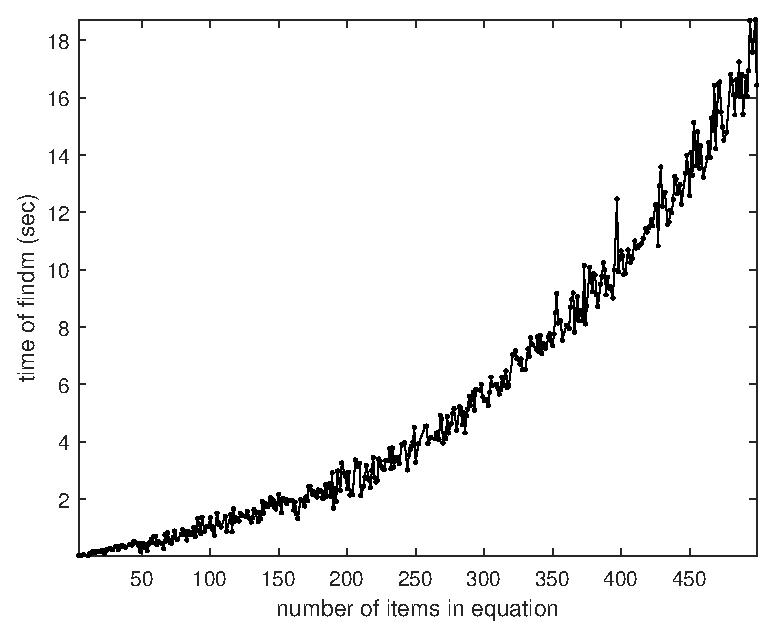
\includegraphics[width=\figwidth]{fig/nlt.eps}
\caption{time complexity}
\label{t-findm}
\end{figure}

Secondly, we are interested in the distribution of BPs. Because there are three types of BPs, and they may occur simultaneously in an equation, we can encode all situations in a binary sequence of length 3. For example, 100 means the equation only has \BPone{}. For the 1000 test equations, the distribution of BPs is shown in \reffig{d-bps}. As we can see, most equations only have \BPone{}. There is no \BPtwo{} in our test. The \BPthree{} only occurs in 4 equations.
\begin{figure}[H]
\centering
\includegraphics[width=\figwidth]{fig/nbps.eps}
\caption{balance points distribution}
\label{d-bps}
\end{figure}

Finally, we are interested in the distribution of the least expansion order. Here 1-order expansion means the equation can be solved by homogeneous balance principle. As we can see in \reffig{d-nexp}, only one case need 2-order expansion. This indicates that very few equations require higher order expansion.
\begin{figure}[H]
\centering
\includegraphics[width=\figwidth]{fig/nexp.eps}
\caption{distribution of minimum expansion order}
\label{d-nexp}
\end{figure}

In summary, experiments show that our algorithm has a polynomial time complexity. Furthermore, \BPtwo{} and \BPthree{} are very rare in our test. Since the rarity of \BPthree{}, there are very few cases need $n$-order expansion. So, 5-order expansion is enough for most cases.

\section{Further discussion about $n$-order expansion method} \label{$n$-order-discussion-02}

Experiments show that 5-order expansion is enough to solve most problems. In this section, we will analyze it theoretically.

In \refsec{Expansion-02}, the power of $n$-order expanded polynomial is calculated by multiplication. But, it is not feasible when the value of power is undetermined. Now, we are going to infer the rule of power operation. According to the properties of powers,
\begin{equation}
\begin{split}
F\sbrace{x,m,u\up n}^h &= \mbrace{\sum_{k=0}^{n-1}{u_kx^{m-k}}+\OO\sbrace{x^{m-n}}}^h \\
&= \sum_{k=0}^{n-1}{\mbrace{\sum_{b_i}{\frac{h!}{\prod_{i=0}^{n-1}{b_i !}}\prod_{i=0}^{n-1}{u_i^{b_i}}}}x^{hm-k}}+\OO\sbrace{x^{hm-n}} \\
&= F\sbrace{x,hm,v\up n}.
\end{split}
\label{power}
\end{equation}
Here, $\mbrace{b_0,\cdots,b_{n-1}}$ is a non-negative integer solution of
\begin{equation}
\sum_{i=0}^{n-1}{b_i}=h,\sum_{i=0}^{n-1}{ib_i}=k \label{bi}.
\end{equation}
When the solution of \refeqn{bi} is determined, we can get the rule of power.

For $0\le k \le n-1$, let
\begin{equation}
S_k=\bbrace{\mbrace{b_0,\cdots,b_{n-1}}\ge 0 \left| \sum_{i=0}^{n-1}{b_i}=h,\sum_{i=0}^{n-1}{ib_i}=k \right.}.
\end{equation}
It is hard to solve $S_k$ when $h$ is undetermined. The key to our approach is to find a finite set $S^*$ that $\bigcup\nolimits_{k=0}^{n-1}S_k\subset S^*$. Then we can filtrate the elements of $S_k$ from $S^*$ in limited steps.

Since
\begin{equation}
\sum_{i=1}^{n-1}{b_i}\le \sum_{i=1}^{n-1}{i b_i}=\sum_{i=0}^{n-1}{i b_i}=k\le n-1,
\end{equation}
we can get
\begin{equation}
\bigcup\limits_{k=0}^{n-1}S_k\subset S=\bbrace{\mbrace{b_0,\cdots,b_{n-1}}\ge 0 \left| \sum_{i=0}^{n-1}{b_i}=h, \sum_{i=1}^{n-1}{b_i}\le n-1 \right.}.
\end{equation}
Obviously, we have
\begin{equation}
S\subset \overline{S}=\bbrace{\mbrace{b_0,\cdots,b_{n-1}}\left|b_0=h-\sum_{i=1}^{n-1}{b_i},b_i=c_i(i\ge 1),\sum_{i=0}^{n-1}c_i=n-1,c_i\ge 0\right.}.
\end{equation}
The scale of $\overline{S}$ is determined by the number of solutions of
\begin{equation}
\sum_{i=0}^{n-1}c_i=n-1 \label{eqc}.
\end{equation}
Since $n$ is limited, $\overline{S}$ is a finite set.  Hence, $\overline{S}$ is the desired set, i.e., we can assign $S^*=\overline{S}$.

Technically, there are $\binom{2n-2}{n-1}$ non-negative integer solutions of \refeqn{eqc}. Assume  $\mbrace{p_1,\cdots,p_{n-1}}$ is a solution of selecting $n-1$ elements from $\bbrace{1,2,\cdots,2n-2}$, let  $p_0=0,p_n=2n-2$, we can get a related solution of \refeqn{eqc} that $c_k=p_{k+1}-p_k-1$.

Finally, we can calculate $v\up n$ of \refeqn{power} in limited steps.

According to the previous inference, when $n=2$, we can get
\begin{equation}
\mbrace{\Delta^r F\sbrace{x,m,u\up 2}}^h=u_0^h x^{mh}+\sbrace{u_0^hm\cdot hr+u_0^{h-1}u_1\cdot h}x^{mh-1}+\OO\sbrace{x^{mh-2}}
\end{equation}
and
\begin{equation}
\begin{split}
&\mbrace{\Delta^{r_1}F\sbrace{x,m,u\up 2}}^{h_1}\cdot \mbrace{\Delta^{r_2}F\sbrace{x,m,u\up 2}}^{h_2}=u_0^{h_1+h_2} x^{m(h_1+h_2)} \\
+&\sbrace{u_0^{h_1+h_2}m\cdot (h_1r_1+h_2r_2)+u_0^{h_1+h_2-1}u_1\cdot (h_1+h_2)}x^{m(h_1+h_2)-1} \\
+&\OO\sbrace{x^{m(h_1+h_2)-2}}.
\end{split}
\end{equation}
Let
\begin{equation}
G\sbrace{h,q;m,u\up 2}=u_0^h x^{mh}+\sbrace{u_0^hm\cdot q+u_0^{h-1}u_1\cdot h}x^{mh-1}+\OO\sbrace{x^{mh-2}},
\end{equation}
we can get
\begin{equation}
\begin{split}
f(x+r)^h=G\sbrace{h,hr;m,u\up 2}&=\mbrace{\Delta^r F\sbrace{x,m,u\up 2}}^h, \\
G\sbrace{h_1,h_1r_1;m,u\up 2}\cdot G\sbrace{h_2,h_2r_2;m,u\up 2}&=G\sbrace{h_1+h_2,h_1r_1+h_2r_2;m,u\up 2}.
\end{split}
\label{key}
\end{equation}
Hence,
\begin{equation}
\begin{split}
\prod_{i=0}^r{f^{\gamma_{ki}}(x+r)}&=\prod_{i=0}^r{G\sbrace{\gamma_{ki},i\gamma_{ki};m,u\up 2}} \\
&=G\sbrace{\sum_{i=0}^r{\gamma_{ki}},\sum_{i=0}^r{i\gamma_{ki}};m,u\up 2} \\
&=G\sbrace{s_k,t_k;m,u\up 2} \\
&=u_0^{s_k} x^{m{s_k}}+\sbrace{u_0^{s_k}m\cdot {t_k}+u_0^{{s_k}-1}u_1\cdot {s_k}}x^{m{s_k}-1}+\OO\sbrace{x^{m{s_k}-2}} .
\end{split}
\end{equation}
Consequently,
\begin{equation}
\begin{split}
& a_k(x)\prod_{i=0}^r{f^{\gamma_{ki}}(x+r)} = \alpha_{k,0}u_0^{s_k} x^{{s_k}m+d_k} \\
+& \mbrace{\alpha_{k,0}\sbrace{u_0^{s_k}m\cdot {t_k}+u_0^{{s_k}-1}u_1\cdot {s_k}}+\alpha_{k,1}u_0^{s_k}}x^{{s_k}m+d_k-1}+\OO\sbrace{x^{{s_k}m+d_k-2}} .
\end{split}
\end{equation}
When $m\ge\underline{m}_2$, we have
\begin{equation}
\begin{split}
\Omega_0&=\sum_{s_k=\sigma,d_k=\delta}{\alpha_{k,0}u_0^{s_k}}=u_0^\sigma\sum_{s_k=\sigma,d_k=\delta}{\alpha_{k,0}} , \\
\Omega_1&=\sum_{s_k=\sigma,d_k=\delta}\mbrace{\alpha_{k,0}\sbrace{u_0^{s_k}m\cdot {t_k}+u_0^{{s_k}-1}u_1\cdot {s_k}}+\alpha_{k,1}u_0^{s_k}}+\sum_{s_k=\sigma,d_k=\delta-1}{\alpha_{k,0}u_0^{s_k}} \\
&=u_0^\sigma m \sum_{s_k=\sigma,d_k=\delta}{\alpha_{k,0}t_k}+u_0^{\sigma-1}u_1\sigma\sum_{s_k=\sigma,d_k=\delta}{\alpha_{k,0}}+u_0^\sigma\sum_{s_k=\sigma,d_k=\delta-1}{\alpha_{k,0}} .
\end{split}
\end{equation}

The invalidation of 2-order expansion requires $\bbrace{\Omega_0=0,\Omega_1=0}$. It is equivalent to
\begin{equation}
\sum_{s_k=\sigma,d_k=\delta}{\alpha_{k,0}}=0,\sum_{s_k=\sigma,d_k=\delta}{\alpha_{k,0}t_k}=0 .\label{invalid}
\end{equation}
\refeqn{invalid} is a system of linear equations with respect to $\alpha_{k,0} (k=1,\cdots,l)$. Assume that there are $r$ items satisfy $s_k=\sigma$ and $d_k=\delta-1$. When $t_k$ are the same, the dimension of solution space is $r-1$. Otherwise, the dimension of solution space is $r-2$. When $r>2$, \refeqn{invalid} may have non-trivial solutions, the 2-order expansion will be invalid.

For higher order expansion, \refeqn{invalid} is also the necessary condition of invalidation. Generally, coefficients $\alpha_{k,0} (k=1,\cdots,l)$ are in a linear space of dimension $r$. The invalidation of $n$-order expansion restrain coefficients in to a sub-space of dimension $r-\epsilon$. Here, $\epsilon\ge 1$. The probability of these situations is 0.

In a word, the larger expansion order, the less probability of invalidation. So, 5-order expansion is enough for most equations.

\section{Conclusion} \label{Conclusion-02}

In conclusion, we developed an algorithm that can find all polynomial solutions for nonlinear difference equations in the form of \refeqn{eq}. Both theoretical analysis and experiments show that the algorithm has a polynomial time complexity, which is efficient in practice. For other forms of equations that can be solved by the homogeneous balance principle, the $n$-order expansion method is also useful for the  exceptional cases.
